\documentclass[12pt]{book}
\setlength{\headheight}{15pt}

\usepackage[margin=1in]{geometry}
\usepackage{color, colortbl}
\usepackage{fancyhdr}
\usepackage{amssymb}
\usepackage{amsmath}
\usepackage{lastpage}
\usepackage{karnaugh-map}
\usepackage{multicol}
\usepackage{graphicx}

\graphicspath{ {./graphics/} }

% begin custom header shit
\pagestyle{fancy}
\fancyhf{}
\lhead{COMP2650 Lecture 10 - Combinational Logic II}
\rhead{Isaac Kilbourne (110043640)}
\rfoot{Page \thepage\ of \pageref{LastPage}}
% end custom header shit

\definecolor{LightRed}{rgb}{1, 0.6, 0.6}
\definecolor{LightGreen}{rgb}{0.6, 1, 0.6}
\newcolumntype{R}{>{\columncolor{LightRed}}c}
\newcolumntype{G}{>{\columncolor{LightGreen}}c}

\newenvironment{indented} {
	\begin{list}{}{\setlength{\leftmargin}{5mm}}
	\item[]
}{\end{list}}
	
\raggedbottom 
\begin{document}
	\noindent
	1. Design a half-subtractor circuit with input $x$ and $y$ and outputs $D$ (Difference) and $B_{out}$ (Borrow)
	which performs $x-y$.
	\begin{indented}
		$\left.\begin{array}{c|c||c|c}
				x & y & D & B_{out} \\
				\hline
				0 & 0 & 0 & 0 \\
				0 & 1 & 1 & 1 \\
				1 & 0 & 1 & 0 \\
				1 & 1 & 0 & 0 \\
		\end{array}
		\right\}
		\begin{aligned}
			D &= x \oplus y\\
			B_{out} &= x'y\\
		\end{aligned}$

		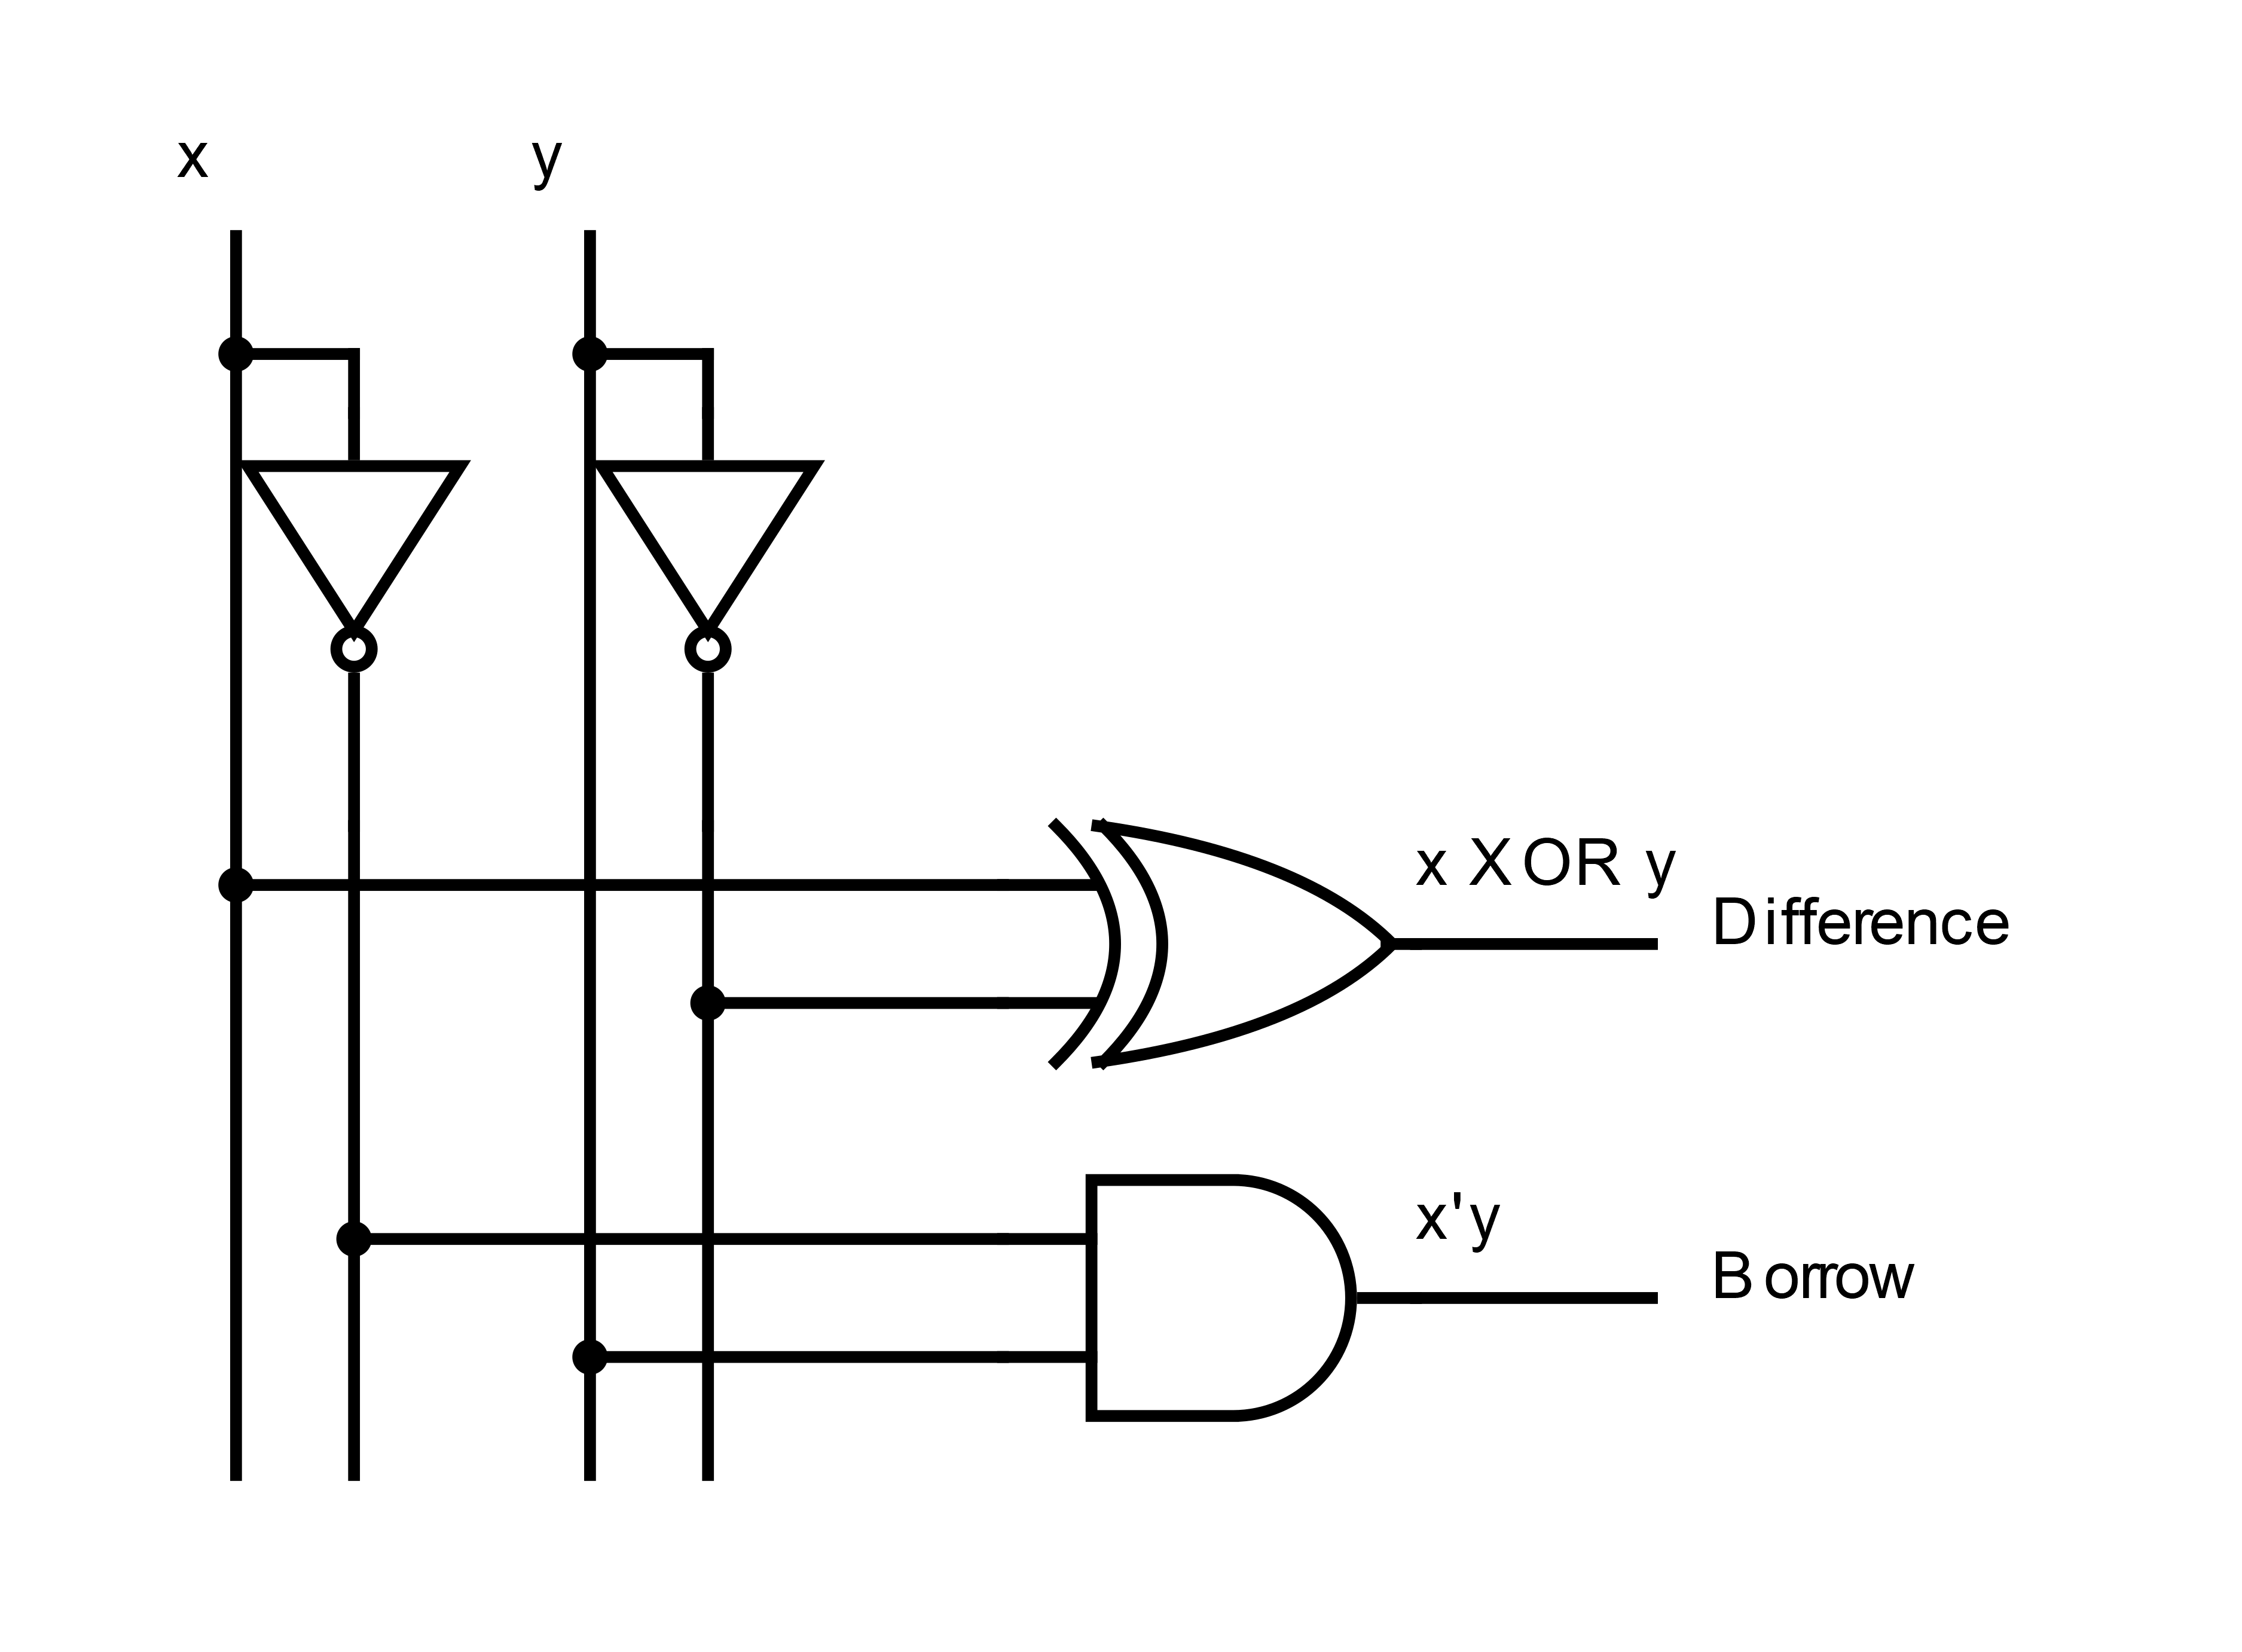
\includegraphics[width=3.5in]{q1_half_subtractor}
	\end{indented}

	\noindent
	2. Design a full-subtractor circuit with three inputs, $x$, $y$, and $B_{prev}$, which performs
	\linebreak $x-y-B_{prev}$.
	\begin{indented}
		$\begin{array}{c|c|c||c|c||c}
			B_{prev} & x & y & D & B_{out}\\
			\hline
			0 & 0 & 0 & 0 & 0 & 0 \\
			0 & 0 & 1 & 1 & 1 & 1 \\
			0 & 1 & 0 & 1 & 0 & 2 \\
			0 & 1 & 1 & 0 & 0 & 3 \\
			1 & 0 & 0 & 1 & 1 & 4 \\
			1 & 0 & 1 & 0 & 1 & 5 \\
			1 & 1 & 0 & 0 & 0 & 6 \\
			1 & 1 & 1 & 1 & 1 & 7 \\
		\end{array}$
	
		\begin{multicols}{2}
			\begin{karnaugh-map}[4][2][1][(D) $xy$][$B_{prev}$]
				\minterms{1, 2, 4, 7}
				\maxterms{0, 3, 5, 6}
				
				\implicant{0}{6}
			\end{karnaugh-map}
			
			\columnbreak
			
			\begin{karnaugh-map}[4][2][1][($B_{out}$) $xy$][$B_{prev}$]
				\minterms{1, 4, 5, 7}
				\maxterms{0, 2, 3, 6}
				
				\implicant{1}{5}
				\implicant{4}{5}
				\implicant{5}{7}
			\end{karnaugh-map}
			\footnotemark
			
			\footnotetext[1]{The package used for drawing kmaps does not support diagonal groups. I have used regular
			a regular 4x2 group in this case, however it should be observed to be representative of XOR, not a larger
			implicant.}
		\end{multicols}

		% from the diagonal pattern (imagine the right half being tiled on top)
		$\therefore D = x \oplus y \oplus B_{prev}$

		$\begin{aligned}
			\therefore B_{out} &= x'y + B_{prev}x' + B_{prev}y\\
			&= B_{prev}(x' + y) + x'y
		\end{aligned}$
	\end{indented}

	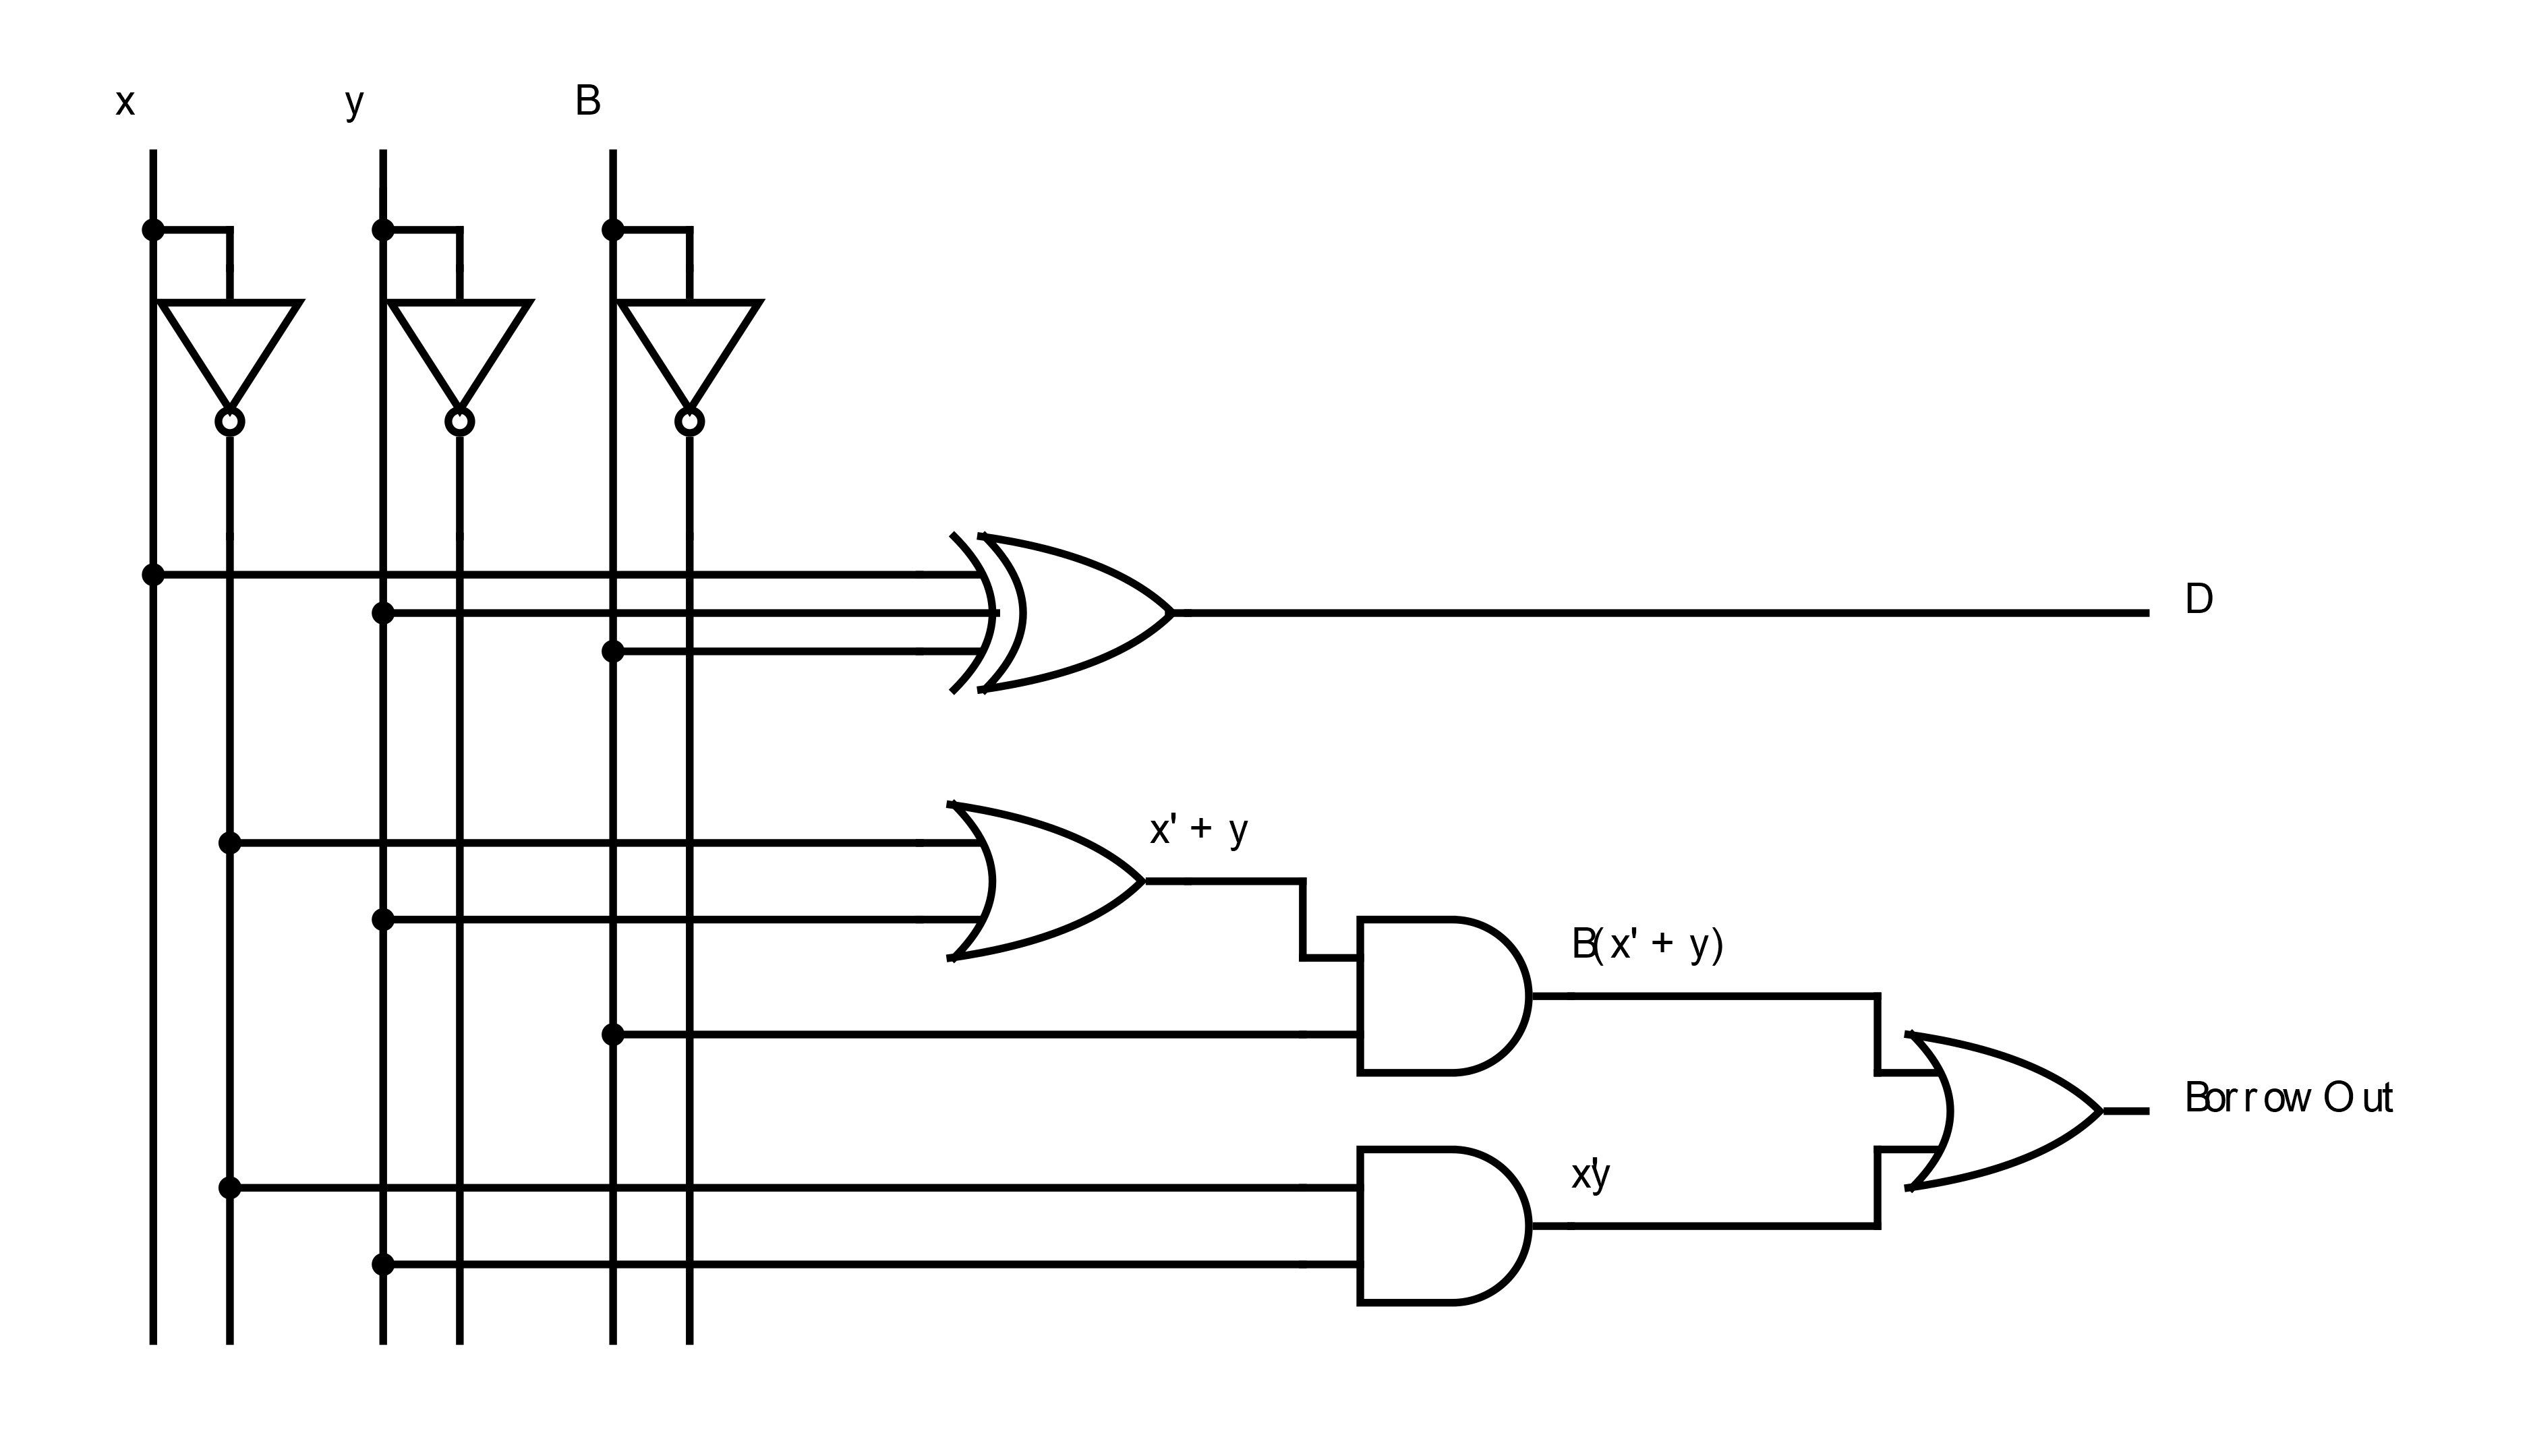
\includegraphics{q2_full_subtractor}

	\footnotetext{The application used to draw these circuits has issues rendering text.
	I apologize for any inconvenience..}
\end{document}
		